\subsection{Multinomial targets}
Now, we consider not only boolean but also multinomial categorical targets. As we already indicated before, we then have a precision and recall value per target class. Let's look at one exemplary confusion matrix.


\begin{figure}[H]
  \centering
  \begin{subfigure}{0.7\textwidth}
    \centering
    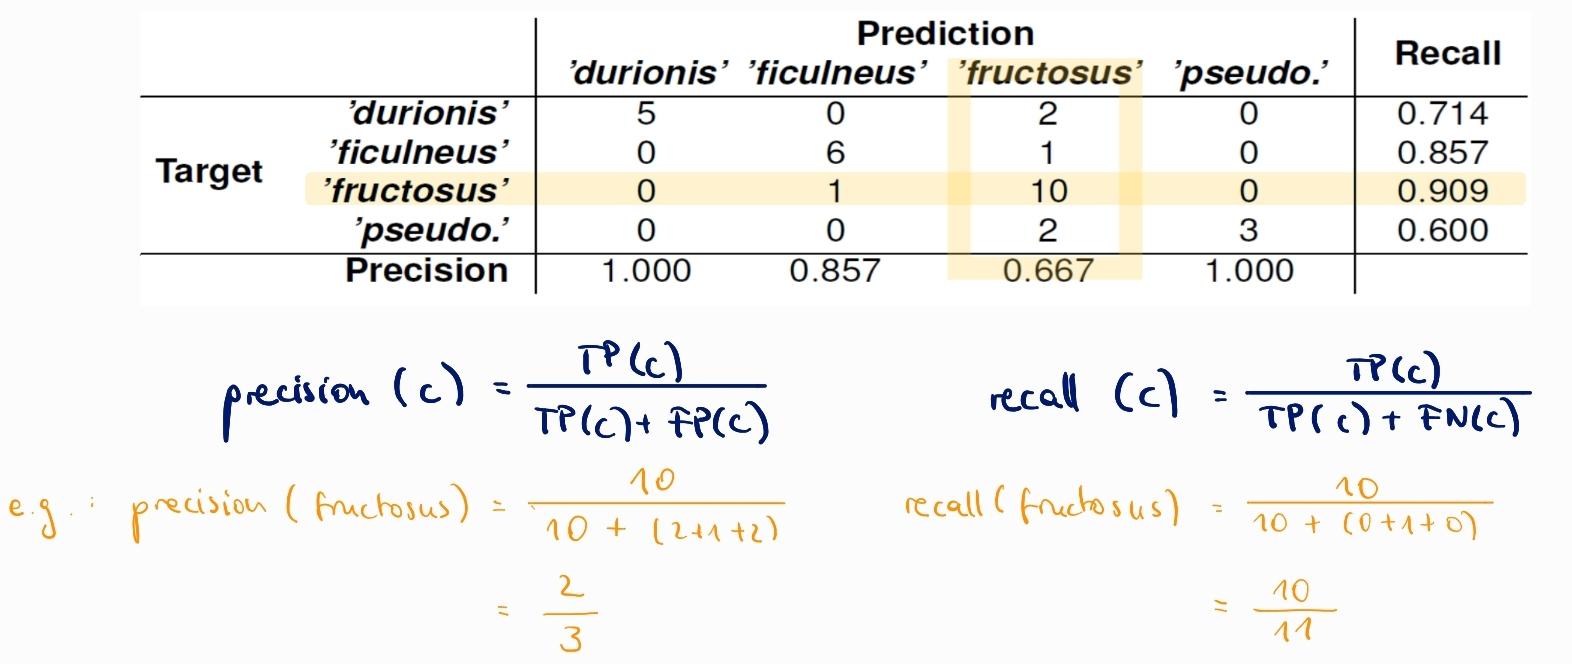
\includegraphics[width=\textwidth]{assets/sl/mt__example.jpg}
  \end{subfigure}

  \caption{Exemplary confusion matrix for multinomial target}
  \label{fig:7_mt_example}
\end{figure}
